%\documentclass[9pt]{scrartcl}
\documentclass[a4paper]{article}
\usepackage[]{amsmath}
\usepackage{tikz}
\usetikzlibrary{positioning}
%\usepackage{helvet}
\usepackage{listings}
\usepackage{geometry}
%\geometry{textheight=\paperheight, noheadfoot, nomarginpar}
\geometry{margin=0.5in}
\usetikzlibrary{positioning,shapes,shadows}
\renewcommand{\familydefault}{\sfdefault}

\tikzstyle{abstract}=[rectangle, draw=black, fill=gray!20, text centered,  text=black, text width=12.5mm]
\tikzstyle{spacestyle}=[rectangle, draw=black, fill=gray!20, text centered,  text=black, text width=50mm]

\lstset{
        language=python,
        basicstyle=\fontencoding{T1}\ttfamily,
        commentstyle=\color{gray},
        keywordstyle=\color{OliveGreen},
        frame=single,
        backgroundcolor=\color{lightlightgray},
        tabsize=2,
        %deletestring=[d]",
        %escapechar=\%,
        numbers=left,
        showstringspaces=false,
}
\usepackage[explicit]{titlesec} 
\titleformat{\section}{\normalfont\Large\bfseries}{}{0em}{#1}
\titleformat{\subsection}{\normalfont\bfseries}{}{0em}{--#1}

\newcommand{\mykey}[2]{%
\begin{tikzpicture} \node (Item) [abstract, minimum size=12.5mm, align=center]
{\vrule height 12pt depth 8pt width 0pt\textbf{#1} \\\vrule height 6pt depth 8pt width 0pt\parbox{1.25cm}{\centering{\fontsize{6pt}{8pt}\selectfont{#2}}}};%
\end{tikzpicture}}


\begin{document}
\begin{center}
\Large{Diagram}
\end{center}
\noindent%


\section {Token ring diagram}
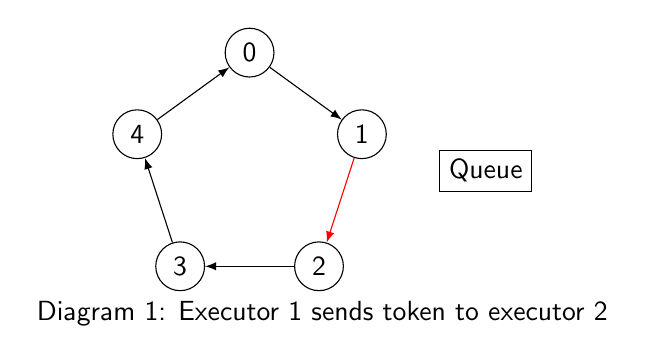
\begin{tikzpicture}

\foreach \i/\number/\color in {0/0/black, 1/1/black, 2/2/black, 3/3/black, 4/4/black} {
    \draw ({90-72*\i}:1.5cm) node[circle,draw=\color] (\number) {\number};
}

\foreach \i/\color in {0/black,1/red,2/black,3/black,4/black} {
    \pgfmathtruncatemacro{\next}{mod(\i+1,5)}
    \draw[draw=\color,-latex] (\i) -- (\next);
}
\node[draw,rectangle] (queue) at (3,0) {Queue};
\node[below] at (current bounding box.south) {Diagram 1: Executor 1 sends token to executor 2};
\end{tikzpicture}\\\\
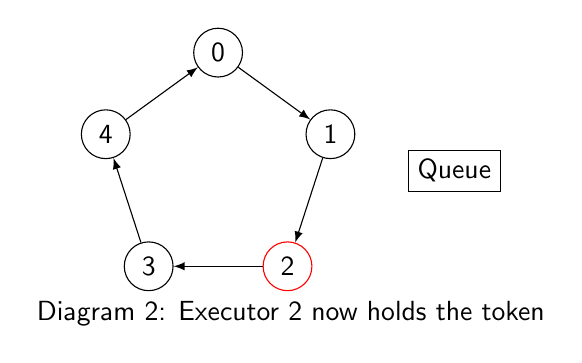
\begin{tikzpicture}

\foreach \i/\number/\color in {0/0/black, 1/1/black, 2/2/red, 3/3/black, 4/4/black} {
    \draw ({90-72*\i}:1.5cm) node[circle,draw=\color] (\number) {\number};
}

\foreach \i in {0,1,2,3,4} {
    \pgfmathtruncatemacro{\next}{mod(\i+1,5)}
    \draw[-latex] (\i) -- (\next);
}
\node[draw,rectangle] (queue) at (3,0) {Queue};
\node[below] at (current bounding box.south) {Diagram 2: Executor 2 now holds the token};
\end{tikzpicture}\\\\
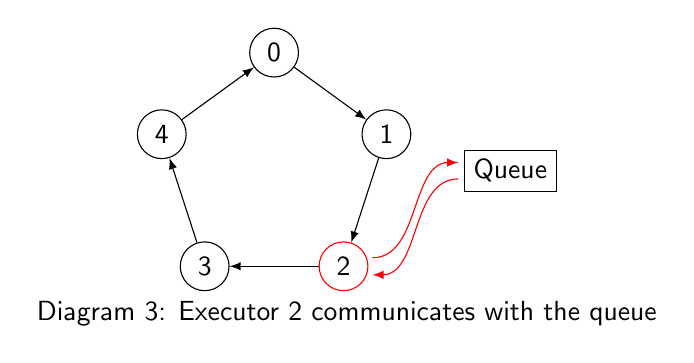
\begin{tikzpicture}

\foreach \i/\number/\color in {0/0/black, 1/1/black, 2/2/red, 3/3/black, 4/4/black} {
    \draw ({90-72*\i}:1.5cm) node[circle,draw=\color] (\number) {\number};
}

\foreach \i in {0,1,2,3,4} {
    \pgfmathtruncatemacro{\next}{mod(\i+1,5)}
    \draw[-latex] (\i) -- (\next);
}

\node[draw,rectangle] (queue) at (3,0) {Queue};
\draw[-latex, red, shorten >=2pt, shorten <=2pt] (2.20) to[out=0, in=180] (queue.170);
\draw[-latex, red, shorten >=2pt, shorten <=2pt] (queue.190) to[out=180, in=0] (2.340);
\node[below] at (current bounding box.south) {Diagram 3: Executor 2 communicates with the queue};
\end{tikzpicture}\\\\
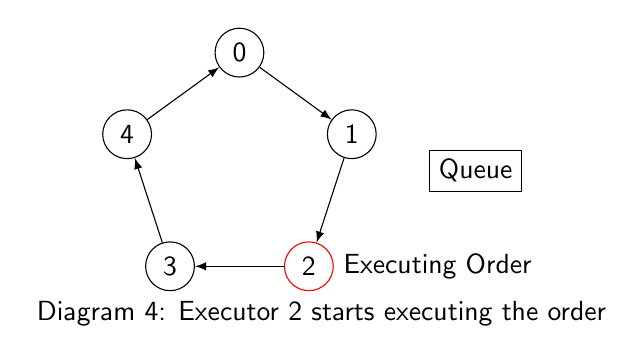
\begin{tikzpicture}

\foreach \i/\number/\color in {0/0/black, 1/1/black, 2/2/red, 3/3/black, 4/4/black} {
    \draw ({90-72*\i}:1.5cm) node[circle,draw=\color] (\number) {\number};
}

\foreach \i in {0,1,2,3,4} {
    \pgfmathtruncatemacro{\next}{mod(\i+1,5)}
    \draw[-latex] (\i) -- (\next);

}
\node[draw,rectangle] (queue) at (3,0) {Queue};
\node[right] at (2.east) {Executing Order};
\node[below] at (current bounding box.south) {Diagram 4: Executor 2 starts executing the order};
\end{tikzpicture}\\\\
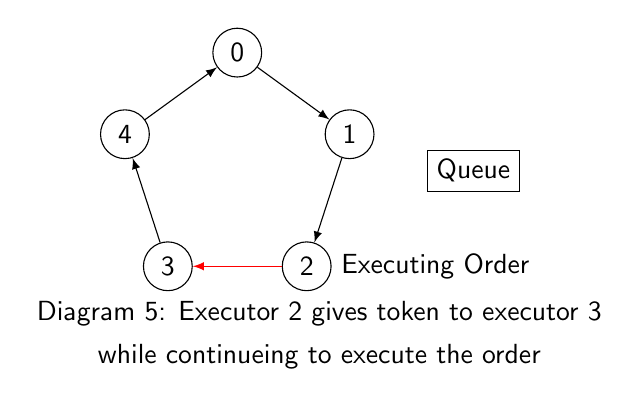
\begin{tikzpicture}

\foreach \i/\number/\color in {0/0/black, 1/1/black, 2/2/black, 3/3/black, 4/4/black} {
    \draw ({90-72*\i}:1.5cm) node[circle,draw=\color] (\number) {\number};
}

\foreach \i/\color in {0/black,1/black,2/red,3/black,4/black} {
    \pgfmathtruncatemacro{\next}{mod(\i+1,5)}
    \draw[draw=\color,-latex] (\i) -- (\next);
}

\node[draw,rectangle] (queue) at (3,0) {Queue};
\node[right] at (2.east) {Executing Order};
\node[below] at (current bounding box.south) {Diagram 5: Executor 2 gives token to executor 3};
\node[below] at (current bounding box.south) {while continueing to execute the order};
\end{tikzpicture}




\section {Resilience to executor death}
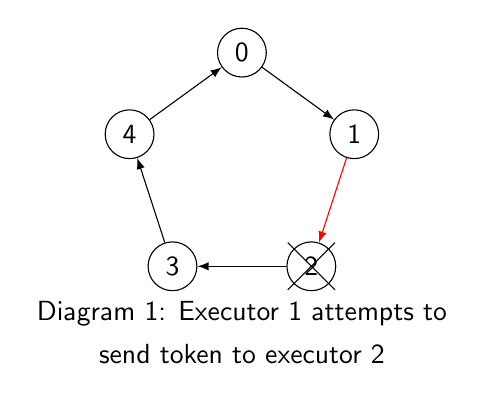
\begin{tikzpicture}

\foreach \i/\number/\color in {0/0/black, 1/1/black, 2/2/black, 3/3/black, 4/4/black} {
    \draw ({90-72*\i}:1.5cm) node[circle,draw=\color] (\number) {\number};
}

\foreach \i/\color in {0/black,1/red,2/black,3/black,4/black} {
    \pgfmathtruncatemacro{\next}{mod(\i+1,5)}
    \draw[draw=\color,-latex] (\i) -- (\next);
}

\draw[black] (2.center) ++ (-0.3, -0.3) -- ++ (0.6, 0.6);
\draw[black] (2.center) ++ (-0.3, 0.3) -- ++ (0.6, -0.6);

\node[below] at (current bounding box.south) {Diagram 1: Executor 1 attempts to};
\node[below] at (current bounding box.south) {send token to executor 2};
\end{tikzpicture}\\\\
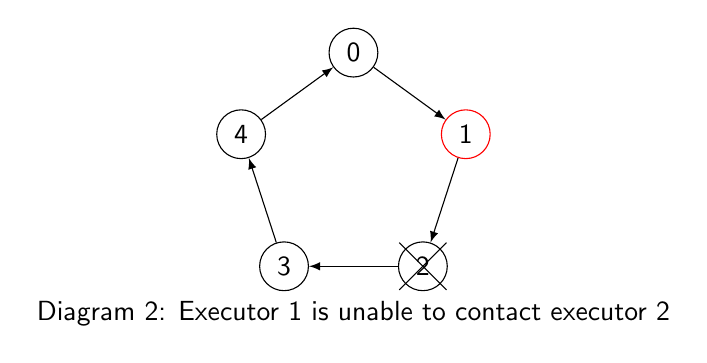
\begin{tikzpicture}

\foreach \i/\number/\color in {0/0/black, 1/1/red, 2/2/black, 3/3/black, 4/4/black} {
    \draw ({90-72*\i}:1.5cm) node[circle,draw=\color] (\number) {\number};
}

\foreach \i in {0,1,2,3,4} {
    \pgfmathtruncatemacro{\next}{mod(\i+1,5)}
    \draw[-latex] (\i) -- (\next);
}

\draw[black] (2.center) ++ (-0.3, -0.3) -- ++ (0.6, 0.6);
\draw[black] (2.center) ++ (-0.3, 0.3) -- ++ (0.6, -0.6);

\node[below] at (current bounding box.south) {Diagram 2: Executor 1 is unable to contact executor 2};
\end{tikzpicture}\\\\
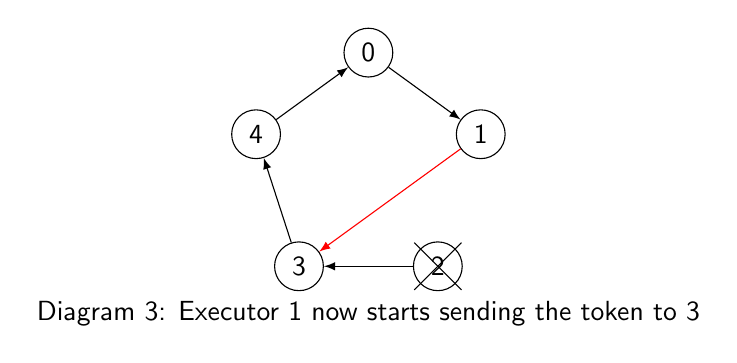
\begin{tikzpicture}

\foreach \i/\number/\color in {0/0/black, 1/1/black, 2/2/black, 3/3/black, 4/4/black} {
    \draw ({90-72*\i}:1.5cm) node[circle,draw=\color] (\number) {\number};
}

\foreach \i in {0,1,2,3,4} {
    \ifnum\i=1
        \pgfmathtruncatemacro{\next}{3}
        \draw[red,-latex] (\i) -- (\next);
    \else
        \pgfmathtruncatemacro{\next}{mod(\i+1,5)}
        \draw[-latex] (\i) -- (\next);
    \fi
}

\draw[black] (2.center) ++ (-0.3, -0.3) -- ++ (0.6, 0.6);
\draw[black] (2.center) ++ (-0.3, 0.3) -- ++ (0.6, -0.6);

\node[below] at (current bounding box.south) {Diagram 3: Executor 1 now starts sending the token to 3};
\end{tikzpicture}

\clearpage


\section {Rejoining the ring}

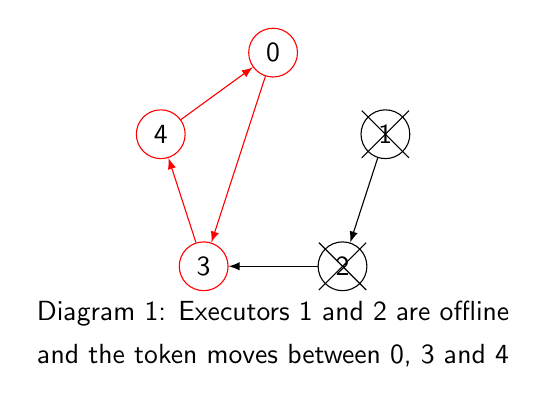
\begin{tikzpicture}

\foreach \i/\number/\color in {0/0/red, 1/1/black, 2/2/black, 3/3/red, 4/4/red} {
    \draw ({90-72*\i}:1.5cm) node[circle,draw=\color] (\number) {\number};
}

\draw[red,-latex] (0) -- (3);
\draw[-latex] (1) -- (2);
\draw[-latex] (2) -- (3);
\draw[red,-latex] (3) -- (4);
\draw[red,-latex] (4) -- (0);

\draw[black] (1.center) ++ (-0.3, -0.3) -- ++ (0.6, 0.6);
\draw[black] (1.center) ++ (-0.3, 0.3) -- ++ (0.6, -0.6);

\draw[black] (2.center) ++ (-0.3, -0.3) -- ++ (0.6, 0.6);
\draw[black] (2.center) ++ (-0.3, 0.3) -- ++ (0.6, -0.6);

\node[below] at (current bounding box.south) {Diagram 1: Executors 1 and 2 are offline};
\node[below] at (current bounding box.south) {and the token moves between 0, 3 and 4};
\end{tikzpicture}\\\\
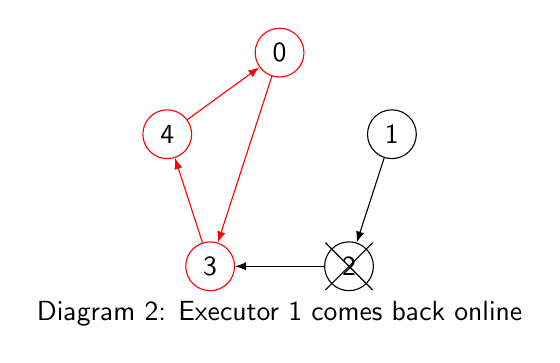
\begin{tikzpicture}

\foreach \i/\number/\color in {0/0/red, 1/1/black, 2/2/black, 3/3/red, 4/4/red} {
    \draw ({90-72*\i}:1.5cm) node[circle,draw=\color] (\number) {\number};
}

\draw[red,-latex] (0) -- (3);
\draw[-latex] (1) -- (2);
\draw[-latex] (2) -- (3);
\draw[red,-latex] (3) -- (4);
\draw[red,-latex] (4) -- (0);

\draw[black] (2.center) ++ (-0.3, -0.3) -- ++ (0.6, 0.6);
\draw[black] (2.center) ++ (-0.3, 0.3) -- ++ (0.6, -0.6);

\node[below] at (current bounding box.south) {Diagram 2: Executor 1 comes back online};

\end{tikzpicture}\\\\
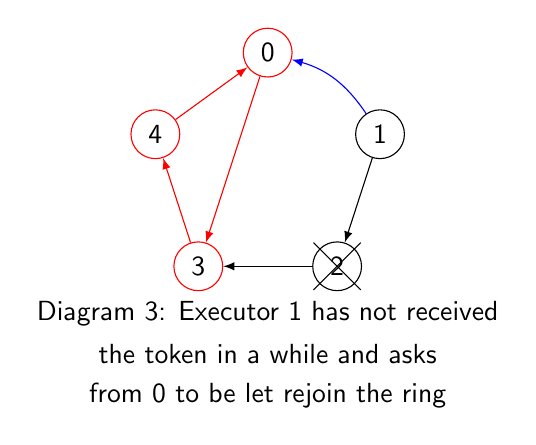
\begin{tikzpicture}

\foreach \i/\number/\color in {0/0/red, 1/1/black, 2/2/black, 3/3/red, 4/4/red} {
    \draw ({90-72*\i}:1.5cm) node[circle,draw=\color] (\number) {\number};
}

\draw[red,-latex] (0) -- (3);
\draw[-latex] (1) -- (2);
\draw[-latex] (2) -- (3);
\draw[red,-latex] (3) -- (4);
\draw[red,-latex] (4) -- (0);

\draw[black] (2.center) ++ (-0.3, -0.3) -- ++ (0.6, 0.6);
\draw[black] (2.center) ++ (-0.3, 0.3) -- ++ (0.6, -0.6);

\draw[blue, -latex, bend right=20] (1) to (0);


\node[below] at (current bounding box.south) {Diagram 3: Executor 1 has not received};
\node[below] at (current bounding box.south) {the token in a while and asks};
\node[below] at (current bounding box.south) {from 0 to be let rejoin the ring};
\end{tikzpicture}\\\\
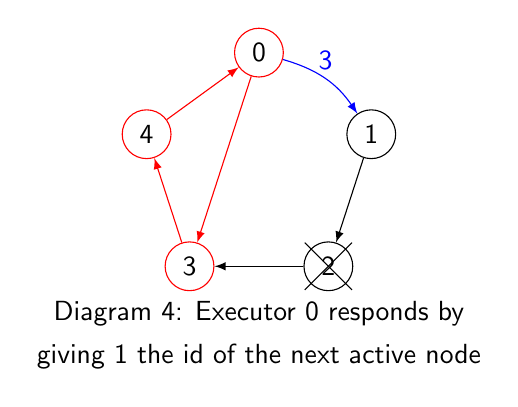
\begin{tikzpicture}

\foreach \i/\number/\color in {0/0/red, 1/1/black, 2/2/black, 3/3/red, 4/4/red} {
    \draw ({90-72*\i}:1.5cm) node[circle,draw=\color] (\number) {\number};
}

\draw[red,-latex] (0) -- (3);
\draw[-latex] (1) -- (2);
\draw[-latex] (2) -- (3);
\draw[red,-latex] (3) -- (4);
\draw[red,-latex] (4) -- (0);

\draw[black] (2.center) ++ (-0.3, -0.3) -- ++ (0.6, 0.6);
\draw[black] (2.center) ++ (-0.3, 0.3) -- ++ (0.6, -0.6);

\draw[blue, -latex, bend left=20] (0) to node[midway, above] {3} (1);


\node[below] at (current bounding box.south) {Diagram 4: Executor 0 responds by};
\node[below] at (current bounding box.south) {giving 1 the id of the next active node};
\end{tikzpicture}\\\\
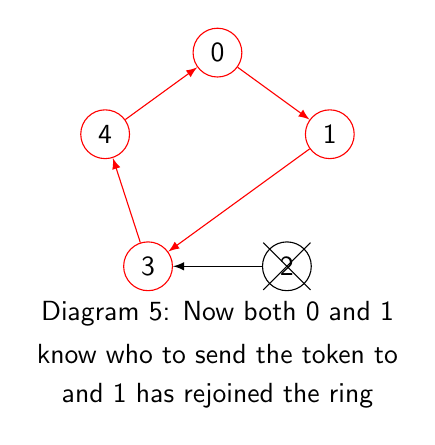
\begin{tikzpicture}

\foreach \i/\number/\color in {0/0/red, 1/1/red, 2/2/black, 3/3/red, 4/4/red} {
    \draw ({90-72*\i}:1.5cm) node[circle,draw=\color] (\number) {\number};
}

\draw[red,-latex] (0) -- (1);
\draw[red,-latex] (1) -- (3);
\draw[-latex] (2) -- (3);
\draw[red,-latex] (3) -- (4);
\draw[red,-latex] (4) -- (0);

\draw[black] (2.center) ++ (-0.3, -0.3) -- ++ (0.6, 0.6);
\draw[black] (2.center) ++ (-0.3, 0.3) -- ++ (0.6, -0.6);



\node[below] at (current bounding box.south) {Diagram 5: Now both 0 and 1};
\node[below] at (current bounding box.south) {know who to send the token to};
\node[below] at (current bounding box.south) {and 1 has rejoined the ring};
\end{tikzpicture}


\end{document}